\RequirePackage{plautopatch}
\documentclass[dvipdfmx,a4paper]{jsarticle}
\usepackage{graphicx}

\usepackage{amsmath}
\usepackage{amssymb}
\usepackage{float}
\usepackage{tikz}
\usepackage{pgfplots}
\pgfplotsset{compat=1.18}
\usepackage{geometry}
\geometry{a4paper, margin=2.5cm} % 余白を設定
\usepackage{listings}     % ソースコードを貼り付けるパッケージ
\usepackage{xcolor}       % コードに色を付ける用
\usepackage{float}
% --- レポートの基本情報 ---
\title{数値解析 期末レポート課題}
\author{大阪大学 工学部 地球総合工学科 \\ 船舶海洋工学コース 08C23031 \\ 古賀\ 光一朗}
\date{2025年8月6日}

% listings (C++コード用) の設定
% カラーテーマと背景色の定義
\definecolor{codegreen}{rgb}{0,0.6,0}
\definecolor{codegray}{rgb}{0.5,0.5,0.5}
\definecolor{codepurple}{rgb}{0.58,0,0.82}
\definecolor{blockbackcolour}{rgb}{0.97,0.97,0.97} %  長いコードブロック用の背景色 (薄いグレー)
\definecolor{inlinebackcolour}{rgb}{0.9,0.9,0.9}   %  短いコード用の背景色 (少し濃いグレー)

% --- 長いコードブロック (\lstinputlisting) の共通設定 ---
\lstset{
    backgroundcolor=\color{blockbackcolour},   % 背景色を薄いグレーに設定
    language=C++,
    basicstyle=\small\ttfamily,
    numbers=left,
    numberstyle=\tiny\color{codegray},
    numbersep=5pt,
    breaklines=true,
    breakatwhitespace=false,
    postbreak=\mbox{\textcolor{red}{$\hookrightarrow$}\space},
    extendedchars=true,
    keywordstyle=\color{blue},
    commentstyle=\color{codegreen},
    stringstyle=\color{codepurple},
    identifierstyle=\color{black},
    frame=tb,
    showstringspaces=false,
    captionpos=b,
}

% 本文中の短いコード用の新コマンドを定義
% \code{...} と書くだけで、背景色が濃いグレーのコードブロックが作れるようにする
\newcommand{\code}[1]{\colorbox{inlinebackcolour}{\lstinline|#1|}}



\begin{document}

\maketitle

使用環境
\begin{itemize}
    \item OS : Windows 10 Home
    \item PC
    \begin{itemize}
        \item CPU : Intel(R) Core(TM) i7-7700T CPU @ 2.90GHz
        \item 実装 RAM : 8.00 GB (7.89 GB 使用可能)
        \item ストレージ : 1.82 TB HDD WDC WD20EZRZ-60Z5HB0, 119 GB SSD SanDisk SD8SMAT-128G-1006
        \item グラフィックス カード : NVIDIA GeForce 930MX (4 GB), Intel(R) HD Graphics 630 (128 MB)
    \end{itemize}
    \item エディタ : Visual Studio Code x64 1.102.3
    \item WSL1 : Ubuntu
    \item 言語 : C++17
    \item グラフ化ソフト : Excel 16.0.19029.20136
    \item 文書作成 : \LaTeX
\end{itemize}

※ matplotのライブラリを読み込んでグラフ描画しようと試みましたが、pythonとWSLがうまく接続できず、断念しました。

※ 変数名等は考えるのは無駄なのでAIに決めさせました。

\section{微分方程式}

\subsection{各種数値解法の精度比較(課題1(ア))}

(ア)微分方程式をオイラー法・ホイン法・ルンゲ・クッタ法で解いたときの“数値精度”を、適切な図を用いてわかりやすく説明しなさい。その際、微分方程式としては振動する2階微分方程式を用い、解析解との比較を行うこと。(50点)

\subsubsection{対象方程式と解法アルゴリズム}
各種数値解法の精度を比較することを考える。そのための具体的なアルゴリズムを以下に示す。

\begin{enumerate}
    \item 比較の基準として、解析解が既知である以下の単振動モデルを対象とする。
    $$
    \frac{d^2 x}{dt^2} = -x
    $$
    初期条件は $x(0) = 1.0$, $\dot{x}(0) = v(0) = 0.0$ とすると、このときの解析解は $x(t) = \cos(t)$ となる。

    \item 数値計算のため、上記の2階微分方程式を、以下の1階連立微分方程式に変換する。
    \begin{align*}
        \frac{dx}{dt} &= v \\
        \frac{dv}{dt} &= -x
    \end{align*}

    \item 時間を$t=0$から$t_{max}$まで、微小な時間刻み幅$\Delta t$で進めながら、各時刻での$x$と$v$の値を求める。この時間発展計算を、以下の3種類の手法でそれぞれ実装する。
    \begin{enumerate}
        \item \textbf{オイラー法:} 現在の時刻$n$における値$(x_n, v_n)$のみを用いて、次時刻$n+1$の値を以下の式で算出する。
        \begin{align*}
            x_{n+1} &= x_n + \Delta t \cdot v_n \\
            v_{n+1} &= v_n + \Delta t \cdot (-x_n)
        \end{align*}

        \item \textbf{ホイン法(2次ルンゲ・クッタ法):} 2段階で計算を行うことで精度を向上させる。
        \begin{enumerate}
            \item まず、オイラー法と同様に次時刻の値を予測する。
            \begin{align*}
                \tilde{x}_{n+1} &= x_n + \Delta t \cdot v_n \\
                \tilde{v}_{n+1} &= v_n + \Delta t \cdot (-x_n)
            \end{align*}
            \item 次に、現在時刻の傾きと予測した時刻の傾きの平均を取り、それを用いて再度計算を行う。
            \begin{align*}
                x_{n+1} &= x_n + \frac{\Delta t}{2} (v_n + \tilde{v}_{n+1}) \\
                v_{n+1} &= v_n + \frac{\Delta t}{2} ((-x_n) + (-\tilde{x}_{n+1}))
            \end{align*}
        \end{enumerate}

        \item \textbf{4次のルンゲ・クッタ法:} 4つの中間的な傾き$k_1, k_2, k_3, k_4$を算出し、それらの加重平均を取ることで極めて高い精度を実現する。各傾きの計算は、課題1(イ)のアルゴリズム説明で詳しく述べるのでそちらを参照されたい。
    \end{enumerate}

    \item 主処理(\code{main}関数)にて、3つの手法による計算結果と解析解を、各時刻ごとにファイルへ出力する。これにより、後のグラフ化による比較が可能となる。
\end{enumerate}


\vspace{5mm}



\subsubsection{計算結果と考察}
図\ref{fig:comparison}に、各手法で得られた数値解と解析解を重ねてプロットしたグラフを示す。

\begin{figure}[H]
    \centering
    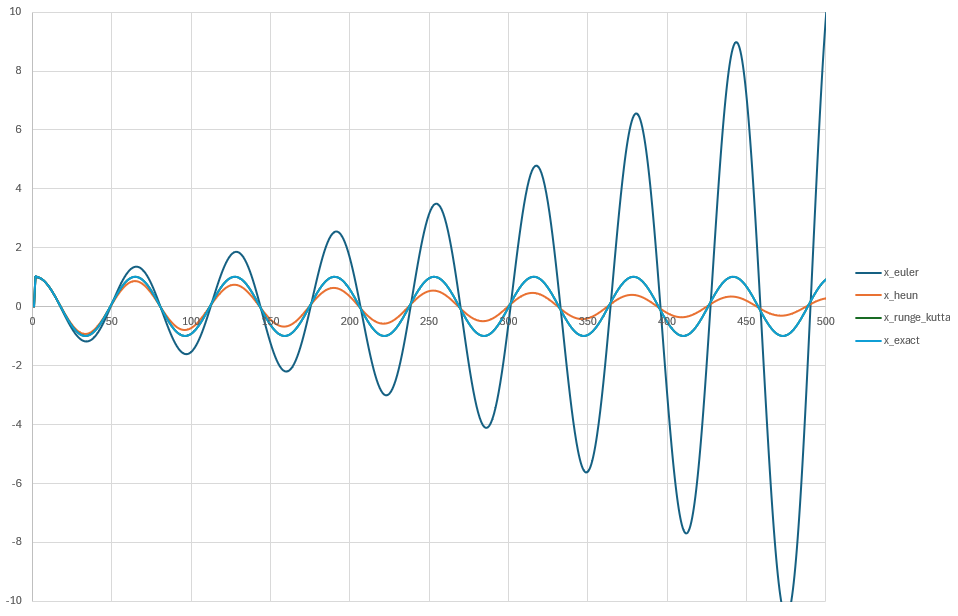
\includegraphics[width=0.9\linewidth]{summer/software-engineering/result_all_methods_01.png} 
    \caption{各種数値解法と解析解の比較}
    \label{fig:comparison}
\end{figure}

図\ref{fig:comparison}から明らかなように、3つの数値解法には顕著な精度の差が見られた。


オイラー法による解(藍色)は、時間経過とともに振幅が増大し、解析解(水色)からの乖離が著しい。これは、各ステップで接線方向に直線的に近似することに起因する累積誤差であると考えられる。


ホイン法による解(橙色)は、オイラー法と比べると大幅に精度が改善されていることがわかる。これは、ステップ内での傾きの予測と修正を行うことで、誤差がある程度抑制できたと考えられる。しかし、長時間の計算では、解析解よりも振幅が小さくなっている。


4次のルンゲ・クッタ法による解(緑色)は、計算範囲の全域にわたって解析解とほぼ完全に一致している。これは、ルンゲ・クッタ法がステップ内で複数点の勾配を評価し、4次のテイラー展開の項まで近似することで、高い精度を実現できたと考えられる。\\
図\ref{fig:comparison}ではルンゲ・クッタ法での誤差が一切確認できない。誤差が見たいので$499.5\leq t \leq 500$の範囲で拡大してみた。(下図\ref{fig:499.5-500})

\begin{figure}[H]
    \centering
    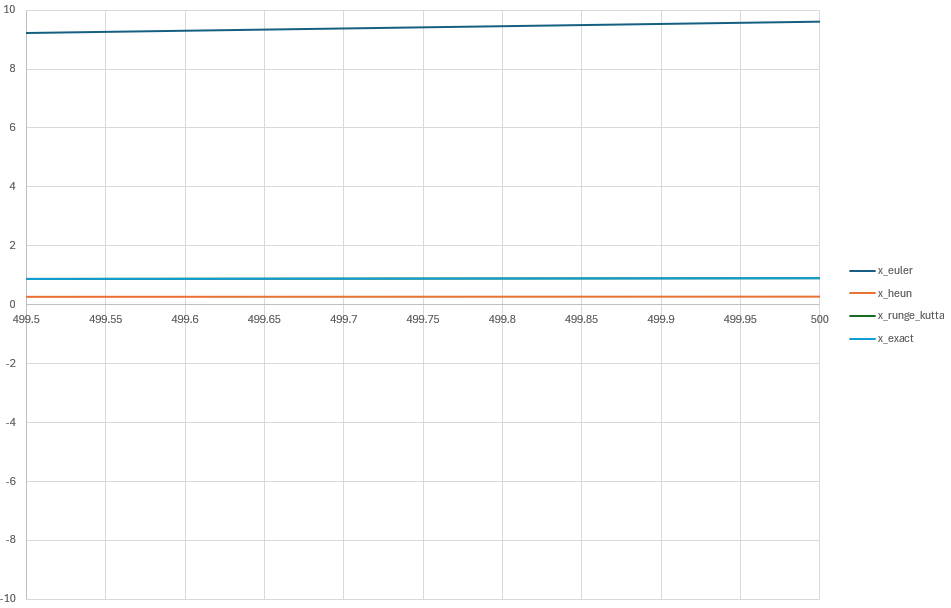
\includegraphics[width=0.5\linewidth]{summer/software-engineering/result_all_methods_02.png}
    \caption{$499.5\leq t \leq 500$での拡大比較}
    \label{fig:499.5-500}
\end{figure}
このように、かなり詳細を確認してもほとんど誤差がない事がわかる。

以上の結果から、振動現象のような解の挙動を長期的に追跡する場合、計算コストが許す限りルンゲ・クッタ法のような高次精度な手法を選択することが重要であるとわかった。

最後に、使用したソースコードを添付する
\lstinputlisting[caption={Source code for Question 1(ア)}, label={lst:code1a}]{3ways.cpp}

\subsection{解の安定性(課題1(イ))}

次の微分方程式を初期値$x_0, \dot{x_0}$について解くことを考える。
$$\ddot{x}+ 0.04455\dot{x} + x − x^3 = B\cos(0.905t)$$
なお、$−1.5 \leq x_0 \leq 1.5$及び$−1.5 \leq \dot{x_0} \leq 1.5$である。いま$B=0$のとき、$t = 0 \sim 100 [s]$まで計算した際、解が発散する初期値の集合を白で描き、解が発散しなかった初期値の集合を黒で描くと次の図のようになっている。このとき、$B$を$0$から徐々に$0.03$ずつ$0.3$まで大きくしていったとき、以下の図はどのように変化するか、図を用いて示しなさい。(20点)

\subsubsection{コードの概要}
外部からの周期的な力(外力)を受ける非線形振動子について、その解の挙動が初期値にどのように依存するかを調べたい。特に、外力の振幅$B$を変化させた際に、解が発散せずに安定な軌道を描く初期値の集合がどのように変化するかを可視化することをめざす。

対象とする微分方程式は、
$$
\ddot{x} + 0.04455\dot{x} + x - x^3 = B \cos(0.905t)
$$
である。これを数値的に解くため、1階の連立微分方程式に変換する。
\begin{align*}
    \frac{dx}{dt} &= v \\
    \frac{dv}{dt} &= -0.04455v - x + x^3 + B \cos(0.905t)
\end{align*}
この方程式を、課題1(ア)で最も精度が高いことを確認した4次のルンゲ・クッタ法を用いて解く。可視化のためのアルゴリズムは以下の通りである。
\begin{enumerate}
    \item 外力の振幅$B$を$0.0$から$0.3$まで$0.03$刻みで変化させるループを設定する。
    \item 各$B$の値に対して、初期値平面($x_0, v_0$)を、それぞれ-1.5から+1.5の範囲で微小なステップ(本実装では0.05)で格子状に区切る。
    \item 格子点の一つ一つを初期値として、ルンゲ・クッタ法により$t=100$まで時間発展計算を行う。
    \item 計算の各ステップで、解の絶対値$|x|$または$|v|$が事前に設定した閾値(100.0)を超えた場合、その解は「発散した」とみなし、その初期値での計算を打ち切る。
    \item $t=100$まで発散しなかった初期値の座標$(x_0, v_0)$のみを、各$B$に対応するファイルに記録する。
\end{enumerate}

\subsubsection{目的とアルゴリズム}
外部からの周期的な力(外力)を受ける非線形振動子について、その解の挙動が初期値にどのように依存するかを調べたい。特に、外力の振幅$B$を変化させた際に、解が発散せずに安定な軌道を描く初期値の集合がどのように変化するかを可視化することをめざす。

対象とする微分方程式は、
$$
\ddot{x} + 0.04455\dot{x} + x - x^3 = B \cos(0.905t)
$$
である。これを数値的に解くため、1階の連立微分方程式に変換する。
\begin{align*}
    \frac{dx}{dt} &= v \\
    \frac{dv}{dt} &= -0.04455v - x + x^3 + B \cos(0.905t)
\end{align*}
この方程式の安定領域を探索するための、具体的なアルゴリズムを以下に示す。

\begin{enumerate}
    \item 4次のルンゲ・クッタ法を用いて、任意の時刻$t$における$(x, v)$から、微小時間$\Delta t$後の値を計算する関数\code{runge_kutta_step()}を定義する。この関数の内部処理は以下の通りである。
    \begin{enumerate}
        \item 現在位置$(t, x, v)$での傾き$k_1$を計算する。
        \item $k_1$を用いて時間$\Delta t/2$だけ進んだ仮の中間点での傾き$k_2$を計算する。
        \item $k_2$を用いて再度、より正確な中間点での傾き$k_3$を計算する。
        \item $k_3$を用いて時間$\Delta t$だけ進んだ仮の終点での傾き$k_4$を計算する。
        \item 4つの傾き$k_1, k_2, k_3, k_4$の加重平均を取り、最終的な次時刻の$(x, v)$の値を更新する。
    \end{enumerate}
    
    \item プログラムの主処理(\code{main}関数)にて、三重ループ構造を用いて安定領域の総当たり探索を行う。
    \begin{enumerate}
        \item 最も外側のループで、外力の振幅$B$を$0.0$から$0.3$まで$0.03$刻みで変化させる。浮動小数点数の誤差を避けるため、ループカウンタは整数とし、ループ内で$B$の値を算出する。
        \item 各$B$の値に対して、初期値平面($x_0, v_0$)を、それぞれ-1.5から+1.5の範囲で微小なステップ(本実装では0.05)で格子状に区切る二重ループを設定する。
        \item 格子点の一つ一つを初期値として、以下の時間発展シミュレーションを行う。
        \begin{enumerate}
            \item 時刻$t=0$から$t_{max}=100$まで、\code{while}ループを用いて計算を繰り返す。
            \item ループの各ステップで、手順1で定義した\code{runge_kutta_step()}関数を呼び出し、$(x, v)$の値を更新する。
            \item 更新後の$x$または$v$の絶対値が、事前に設定した閾値(100.0)を超えた場合、その解は「発散した」とみなし、\code{break}文で\code{while}ループを強制的に終了する。
        \end{enumerate}
        \item \code{while}ループが途中で中断されず、最後まで($t=100$まで)完走した場合のみ、その初期値$(x_0, v_0)$を「安定」とみなし、現在の$B$に対応するファイルに座標を記録する。
    \end{enumerate}
\end{enumerate}


\subsubsection{実行結果と考察}
得られた11個の安定な初期値の集合をそれぞれ散布図としてプロットした。結果を図\ref{fig:basin_b000}から図\ref{fig:basin_b030}に示す。

\begin{figure}[H]
    \centering
    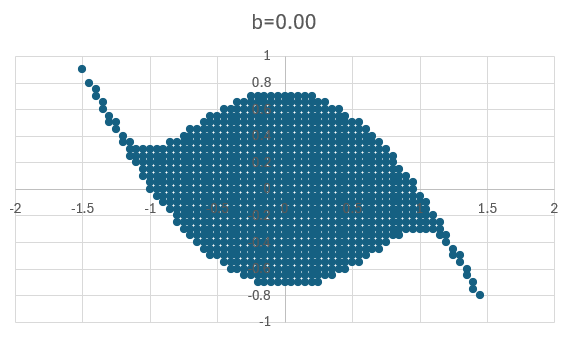
\includegraphics[width=0.45\linewidth]{summer/software-engineering/images/b0.png}
    \caption{$B=0.00$の安定領域}
    \label{fig:basin_b000}
\end{figure}
\begin{figure}[H]
    \centering
    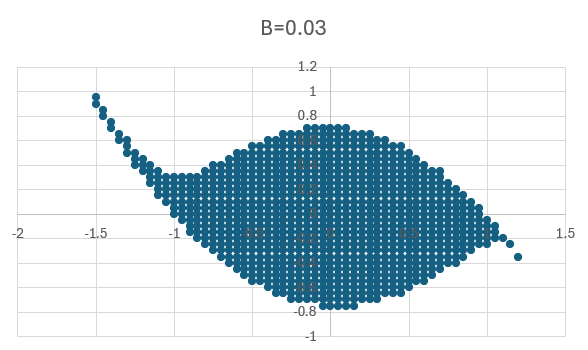
\includegraphics[width=0.45\linewidth]{summer/software-engineering/images/b0.03.png}
    \caption{$B=0.03$の安定領域}
    \label{fig:basin_b003}
\end{figure}
\begin{figure}[H]
    \centering
    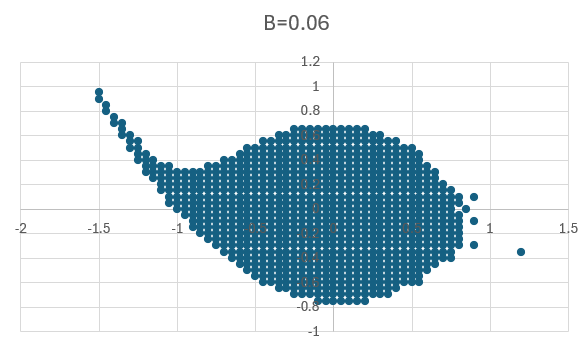
\includegraphics[width=0.45\linewidth]{summer/software-engineering/images/b0.06.png}
    \caption{$B=0.06$の安定領域}
    \label{fig:basin_b006}
\end{figure}
\begin{figure}[H]
    \centering
    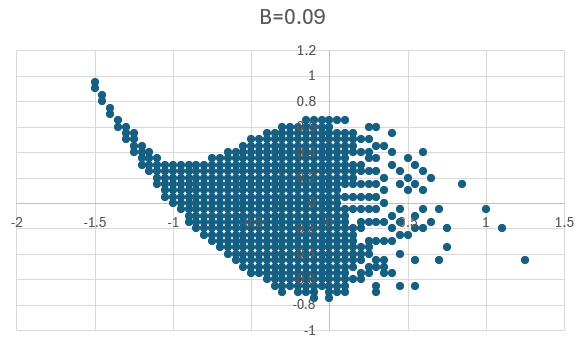
\includegraphics[width=0.45\linewidth]{summer/software-engineering/images/b0.09.png}
    \caption{$B=0.09$の安定領域}
    \label{fig:basin_b009}
\end{figure}
\begin{figure}[H]
    \centering
    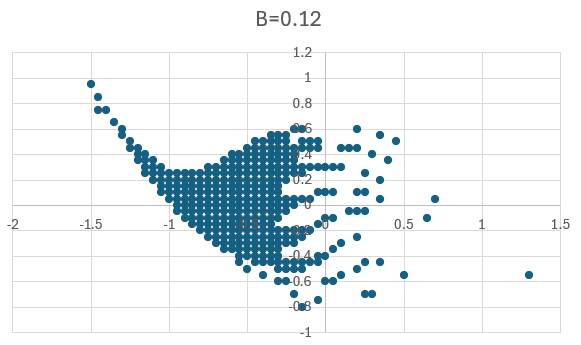
\includegraphics[width=0.45\linewidth]{summer/software-engineering/images/b0.12.png}
    \caption{$B=0.12$の安定領域}
    \label{fig:basin_b012}
\end{figure}
\begin{figure}[H]
    \centering
    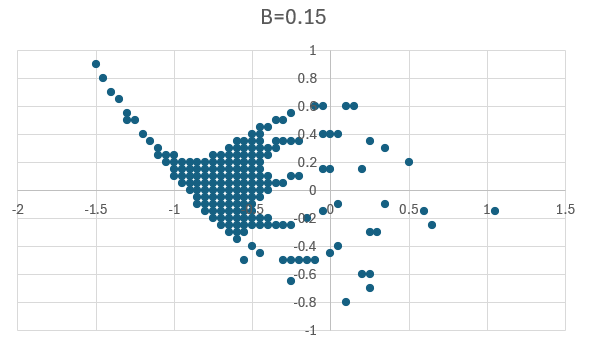
\includegraphics[width=0.45\linewidth]{summer/software-engineering/images/b0.15.png}
    \caption{$B=0.15$の安定領域}
    \label{fig:basin_b015}
\end{figure}
\begin{figure}[H]
    \centering
    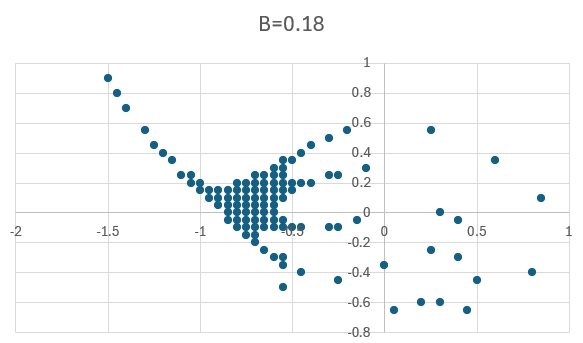
\includegraphics[width=0.45\linewidth]{summer/software-engineering/images/b0.18.png}
    \caption{$B=0.18$の安定領域}
    \label{fig:basin_b018}
\end{figure}
\begin{figure}[H]
    \centering
    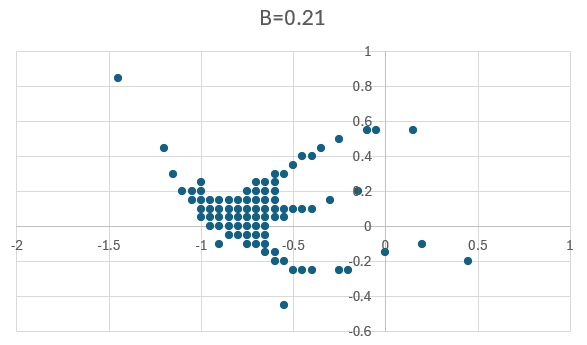
\includegraphics[width=0.45\linewidth]{summer/software-engineering/images/b0.21.png}
    \caption{$B=0.21$の安定領域}
    \label{fig:basin_b021}
\end{figure}
\begin{figure}[H]
    \centering
    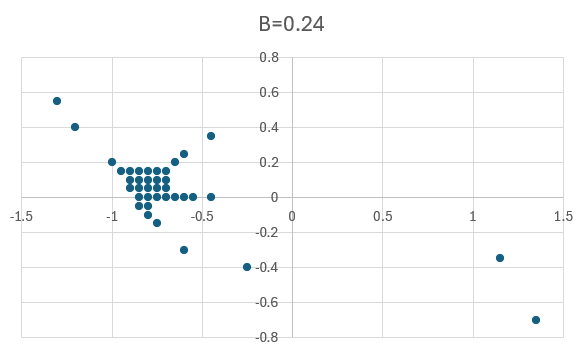
\includegraphics[width=0.45\linewidth]{summer/software-engineering/images/b0.24.png}
    \caption{$B=0.24$の安定領域}
    \label{fig:basin_b024}
\end{figure}
\begin{figure}[H]
    \centering
    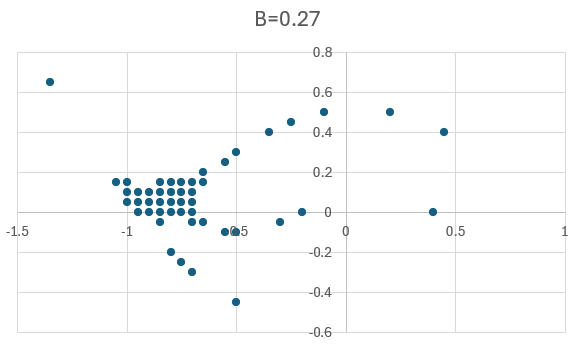
\includegraphics[width=0.45\linewidth]{summer/software-engineering/images/b0.27.png}
    \caption{$B=0.27$の安定領域}
    \label{fig:basin_b027}
\end{figure}
\begin{figure}[H]
    \centering
    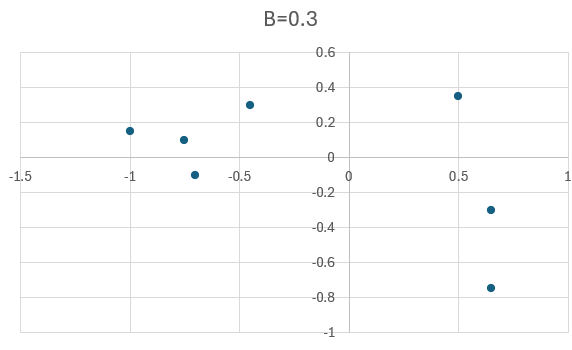
\includegraphics[width=0.45\linewidth]{summer/software-engineering/images/b0.3.png}
    \caption{$B=0.30$の安定領域}
    \label{fig:basin_b030}
\end{figure}

図中の点が、発散しなかった安定な初期値(安定領域)を示している。
$B=0.00$(図\ref{fig:basin_b000})では、課題の参考図と同様に、原点を中心とした大きな安定領域が確認できる。
しかし、外力の振幅$B$が大きくなるにつれて、$B=0.03$から$B=0.09$にかけて(図\ref{fig:basin_b003}〜\ref{fig:basin_b009})、領域の境界が歪み始め、内部に解が発散する領域が現れ始め、
さらに$B$が大きくなると、$B=0.21$(図\ref{fig:basin_b021})あたりから安定領域は著しく侵食され、最終的に$B=0.30$(図\ref{fig:basin_b030})ではほとんど安定領域がうしなわれてしまうことがわかる。


最後に、使用したソースコードを添付する
\lstinputlisting[caption={Source code for Question 1(イ)}, label={lst:code1b}]{runge_kutta_01.cpp}

\section{ニュートン法}

\subsection{4次方程式の求根(課題2(ア))}
4次方程式の4つの解をニュートン法によりすべて見つけるプログラムを作成し、その結果とアルゴリズムを説明しなさい。(15点)
\subsubsection{概要}
ニュートン法を用い、与えられた4次方程式の4つの実数解を自動的にすべて探索するプログラムを作成したい。

ニュートン法の更新式は以下で与えられる。
$$
x_{n+1} = x_n - \frac{f(x_n)}{f'(x_n)}
$$
この反復計算により、単一の初期値から一つの解を見出すことができる。しかし、本課題の目的は「すべての解を見つける」ことであるため、単一の初期値からの計算では不十分である(一敗)。

そこで、本プログラムでは以下の自動探索アルゴリズムを実装した。
\begin{enumerate}
    \item 任意の4次方程式$f(x)=ax^4+bx^3+cx^2+dx+e$と、その導関数$f'(x)$を計算する関数を定義する。

    \item ニュートン法の単一計算を実行し、その成否を真偽値(\code{bool}型)で返す関数\code{newton()}を定義する。この関数の内部処理は以下の通りである。
    \begin{enumerate}
        \item 引数として、計算の出発点となる初期値\code{initial_x}と、計算結果を格納するための変数\code{root_result}への参照を受け取る。
        \item ニュートン法の更新式 $x_{n+1} = x_n - f(x_n)/f'(x_n)$ を、所定の最大回数(本実装では50回)まで反復計算する。
        \item 反復の各ステップで、分母となる$f'(x_n)$の絶対値が極小値($10^{-12}$)より小さいかを判定する。もし小さければ、計算が不安定とみなし、\code{false}を返して関数を終了する。
        \item 更新量$dx = f(x_n)/f'(x_n)$の絶対値が、収束判定の閾値($10^{-9}$)より小さくなったかを判定する。もし小さければ、解が収束したとみなし、計算結果を引数の\code{root_result}に格納した上で、\code{true}を返して関数を終了する。
        \item 最大反復回数に達しても収束しなかった場合、\code{false}を返して関数を終了する。
    \end{enumerate}

    \item プログラムの主処理(\code{main}関数)にて、4つの解を自動で探索する。
    \begin{enumerate}
        \item 発見したユニークな解を保存するためのリスト(\code{std::vector})を空の状態で用意する。
        \item ユーザーから係数$a, b, c, d, e$と、初期値の探索範囲(最小値$x_{min}$, 最大値$x_{max}$)を入力として受け取る。
        \item $x_{min}$から$x_{max}$まで、一定の刻み幅(本実装では0.5)で初期値を変化させながら、以下の処理を繰り返す。
        \item 各初期値に対して、手順2で定義した\code{newton()}関数を呼び出す。
        \item \code{newton()}関数が\code{true}を返した場合のみ、以下の新規性の判定処理に進む。
        \item 得られた解が、すでに解のリストに保存されているものと重複していないかを判定する。具体的には、リスト内の各解と今回得られた解との差の絶対値が、所定の許容誤差($10^{-6}$)よりも大きいかを調べる。
        \item すべての既存の解との差が許容誤差よりも大きかった場合、その解を「新しい解」とみなし、解のリストに追加する。
        \item 解のリストの要素数が4つになった時点で、すべての解が発見されたとみなし、探索の繰り返しを終了する。
    \end{enumerate}
    
    \item 最終的にリストに保存されたすべての解を表示する。
\end{enumerate}
このアルゴリズムにより、自律的に複数の解を発見することができる

\subsubsection{実行結果と考察}
実験として解が $x=1, 2, 3, 4$ となる方程式 
$$f(x) = (x-1)(x-2)(x-3)(x-4)=x^4 - 10x^3 + 35x^2 - 50x + 24 = 0$$
の解探索を実行した。

ソースコードをビルドすると下図\ref{fig:newton-cin2}のように表示されるので
\begin{figure}[H]
\centering
    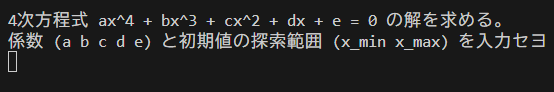
\includegraphics[width=0.7\linewidth]{summer/software-engineering/newton-cin3.png}
    \caption{入力待ち画面}
    \label{fig:newton-cin2}
\end{figure}


1 -10 35 -50 24

-5 5

のように入力すると(※すべての数字の間に空白を入れる)

下図\ref{fig:newton_output_01}のような結果が得られる。

\begin{figure}[H]
    \centering
    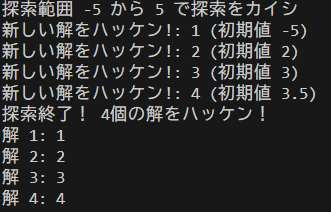
\includegraphics[width=0.5\linewidth]{summer/software-engineering/newton-result_03.png}
    \caption{出力結果}
    \label{fig:newton_output_01}
\end{figure}
よって4解は1,2,3,4であることがわかった。\\
\vspace{5mm}

この結果は、実装した自動探索アルゴリズムが、ニュートン法を繰り返し適用することで4次方程式のすべての実数解を効率的に見つけ出す上で有効であることを示している。

最後に、使用したソースコードを添付する
\lstinputlisting[caption={Source code for Question 2(a)}, label={lst:code2a}]{newton04.cpp}

\subsection{複素平面における収束領域(課題2(イ))}

複素変数$Z$について、以下の方程式をニュートン法で解いたとき、3 つの解のうち、$Z=1$に最終的に行き着く初期値の集合を求め、複素平面上にその集合を図示しなさい。(15点)

$$Z^3-1=0$$

\subsubsection{概要とアルゴリズム}
ニュートン法を複素数領域に拡張し、特定の方程式の解に対する収束領域を可視化することをめざす。

対象となる方程式は、
$$
Z^3 - 1 = 0
$$
この方程式は、複素平面上に次の3解を持つ。
\begin{align*}
    Z_1 &= 1 \\
    Z_2 &= -\frac{1}{2} + i \frac{\sqrt{3}}{2} \\
    Z_3 &= -\frac{1}{2} - i \frac{\sqrt{3}}{2}
\end{align*}
複素数版ニュートン法の更新式は、実数の場合と同様に以下で与えられる。
$$
Z_{n+1} = Z_n - \frac{f(Z_n)}{f'(Z_n)} = Z_n - \frac{Z_n^3 - 1}{3Z_n^2}
$$
可視化のための具体的なアルゴリズムを以下に示す。
\begin{enumerate}
    \item 複素数$Z$を引数に取り、$f(Z)=Z^3-1$およびその導関数$f'(Z)=3Z^2$を計算する関数をそれぞれ定義する。C++の標準ライブラリである\code{<complex>}を用いることで、実数の場合と同様の演算子(\code{+}, \code{-}, \code{*}, \code{/})で計算が可能である。

    \item ニュートン法の単一計算を実行し、どの解に収束したかを整数値で返す関数\code{newton()}を定義する。この関数の内部処理は以下の通りである。
    \begin{enumerate}
        \item 引数として、計算の出発点となる複素数の初期値\code{initial_z}を受け取る。
        \item ニュートン法の更新式 $Z_{n+1} = Z_n - f(Z_n)/f'(Z_n)$ を、所定の最大回数(本実装では50回)まで反復計算する。
        \item 反復の各ステップで、計算結果の$Z_n$が解($f(Z_n) \approx 0$)に十分に近づいたかをまず判定する。
        \item 十分に近づいたと判断された場合、その$Z_n$が3つの既知の解$Z_1, Z_2, Z_3$のうち、どれに最も近いかを、それぞれの解との距離(絶対値)を計算することで判定する。
        \item 最も近い解が$Z_1$であれば\code{1}を、$Z_2$であれば\code{2}を、$Z_3$であれば\code{3}を返し、関数そのものを終了する。どの解にも近くなかった場合は\code{0}を返す。
        \item 最大反復回数に達しても収束しなかった場合も、\code{0}を返して関数を終了する。
    \end{enumerate}

    \item プログラムの主処理(\code{main}関数)にて、解$Z_1=1$の吸引域に属する初期値の集合を探索する。
    \begin{enumerate}
        \item 複素平面上の一定領域(本実装では実部、虚部ともに-2.0から+2.0)を、微小なステップ(0.01)で格子状に区切る二重ループを設定する。
        \item 格子点の一つ一つを複素数の初期値として、手順2で定義した\code{newton()}関数を呼び出す。
        \item \code{newton()}関数から返された値が、本課題の要求する解に対応する\code{1}であった場合のみ、そのときの初期値の座標(実部と虚部)をファイルに出力する。
    \end{enumerate}
\end{enumerate}


\subsubsection{実行結果と考察}
得られた初期値の集合を散布図としてプロットした結果を図\ref{fig:newton_fractal}に示す。

\begin{figure}[htbp]
    \centering
    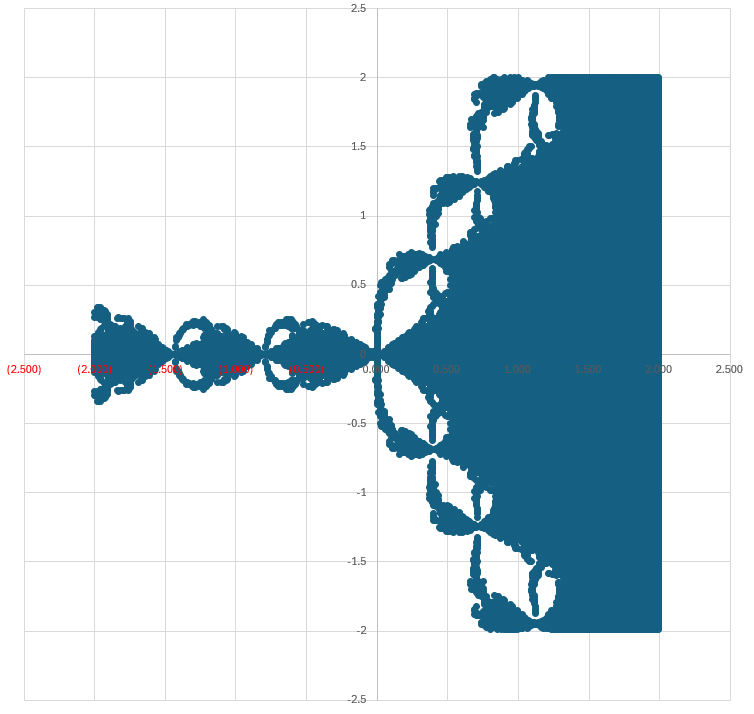
\includegraphics[width=0.8\linewidth]{summer/software-engineering/newton_fractal.png} 
    \caption{方程式 $Z^3-1=0$ の解 $Z=1$ に対する吸引域}
    \label{fig:newton_fractal}
\end{figure}

図\ref{fig:newton_fractal}は、解$Z=1$に収束する初期値の集合、を示している。この図から、実軸上の正の領域に広がる主要な領域のほか、他の解の吸引域の内部にまで複雑に入り込んでいる様子が確認できる。
このように、異なる解の吸引域の境界線が単純な線ではなく、無限に入り組んだ複雑な形状をなす構造は\textbf{ニュートンフラクタル}として知られている。



最後に、使用したソースコードを添付する
\lstinputlisting[caption={Source code for Question 2(イ)}, label={lst:code2b}]{complex_newton_01.cpp}


\end{document}
